\chapter{Introduction}

\section{Particle Accelerators}

Particle accelerators are widely used in scientific research; they are facilities where a variety of experiments can be performed, including some using photon beams.
Experiments involving photon beams generally involve using the beam to strike a target material or sample to study its properties.
There are two main architectures for building particle accelerators:

\begin{itemize}
    \item linear accelerators (in-line).
    \item circular accelerators (synchrotrons).
\end{itemize}

A synchrotron is compose by different parts:

\begin{itemize}
    \item Linear accelerator: This is where the electrons begin their journey by acquiring velocity near the speed of light.
    \item Booster ring: After the linear accelerators, the electrons end up in a small ring where they gain energy until a threshold.
    \item Storage ring: After reaching the threshold energy, the electrons are injected into the storage ring where they maintain their energy for a long time.
\end{itemize}

The storage ring is composed by multiple straight segments, this imply the presence of angles between them.
The beam of electrons is steered by bending magnets from one segment to the other and by doing this they emit synchrotron radiation photons.
In this way is possible to route the photons into experimental stations called beamlines.
The beam need to be positioned correctly during the experiments and keep it in the right position.
Beam position monitors (BPMs) are used to locate the beam, they are minimally invasive type of device.
Once the position is known, a control system can be used to adjust the position of the beam so that it is at the target location.
The control system is able to modify the position of the beam by acting on the piezoelectric actuators and must do so continuously.\cite{Proux2006,Stoupin2010}.
Piezoelectric devices operate by applying voltage and, as they move, change the position of the crystals of the double crystal monochromator (DCM), the main purpose of which is to select the wavelength.
However, the crystals must be aligned with each other, otherwise the intensity of the beam would be negatively affected.
To understand the correct angle (operating point) to keep between the two crystals of the monochromator, the profile of the rocking curve is traced, thus allowing the peak of the beam intensity to be identified.
The operating point may vary over time, thus for continuously target the peak intensity, its own location must be tracked  for optimal experimental throughput \cite{vanSilfhout2014,Quinn2021}. 

\section{Peak Intensity Misalignment}

Each synchrotron beamline requires customized equipment to acquire beam data, move its components, and apply corrections to the components while performing experiments.
Although the components of a beamline are not independent of each other, some of them have more influence on the intensity of the beam.
These are called double crystal monochromators (DCM). 
The component is composed of two crystals and must be correctly aligned, as misalignment would lead to a degradation of the beam intensity.
Based on the angle between the two crystals of the monochromator, it is possible to measure the intensity obtained. Mapping the angle with the intensity produced by the beam produces a profile called a rocking curve [~\ref{fig:rocking curve}].

\begin{figure}[htbp]
    \centering
    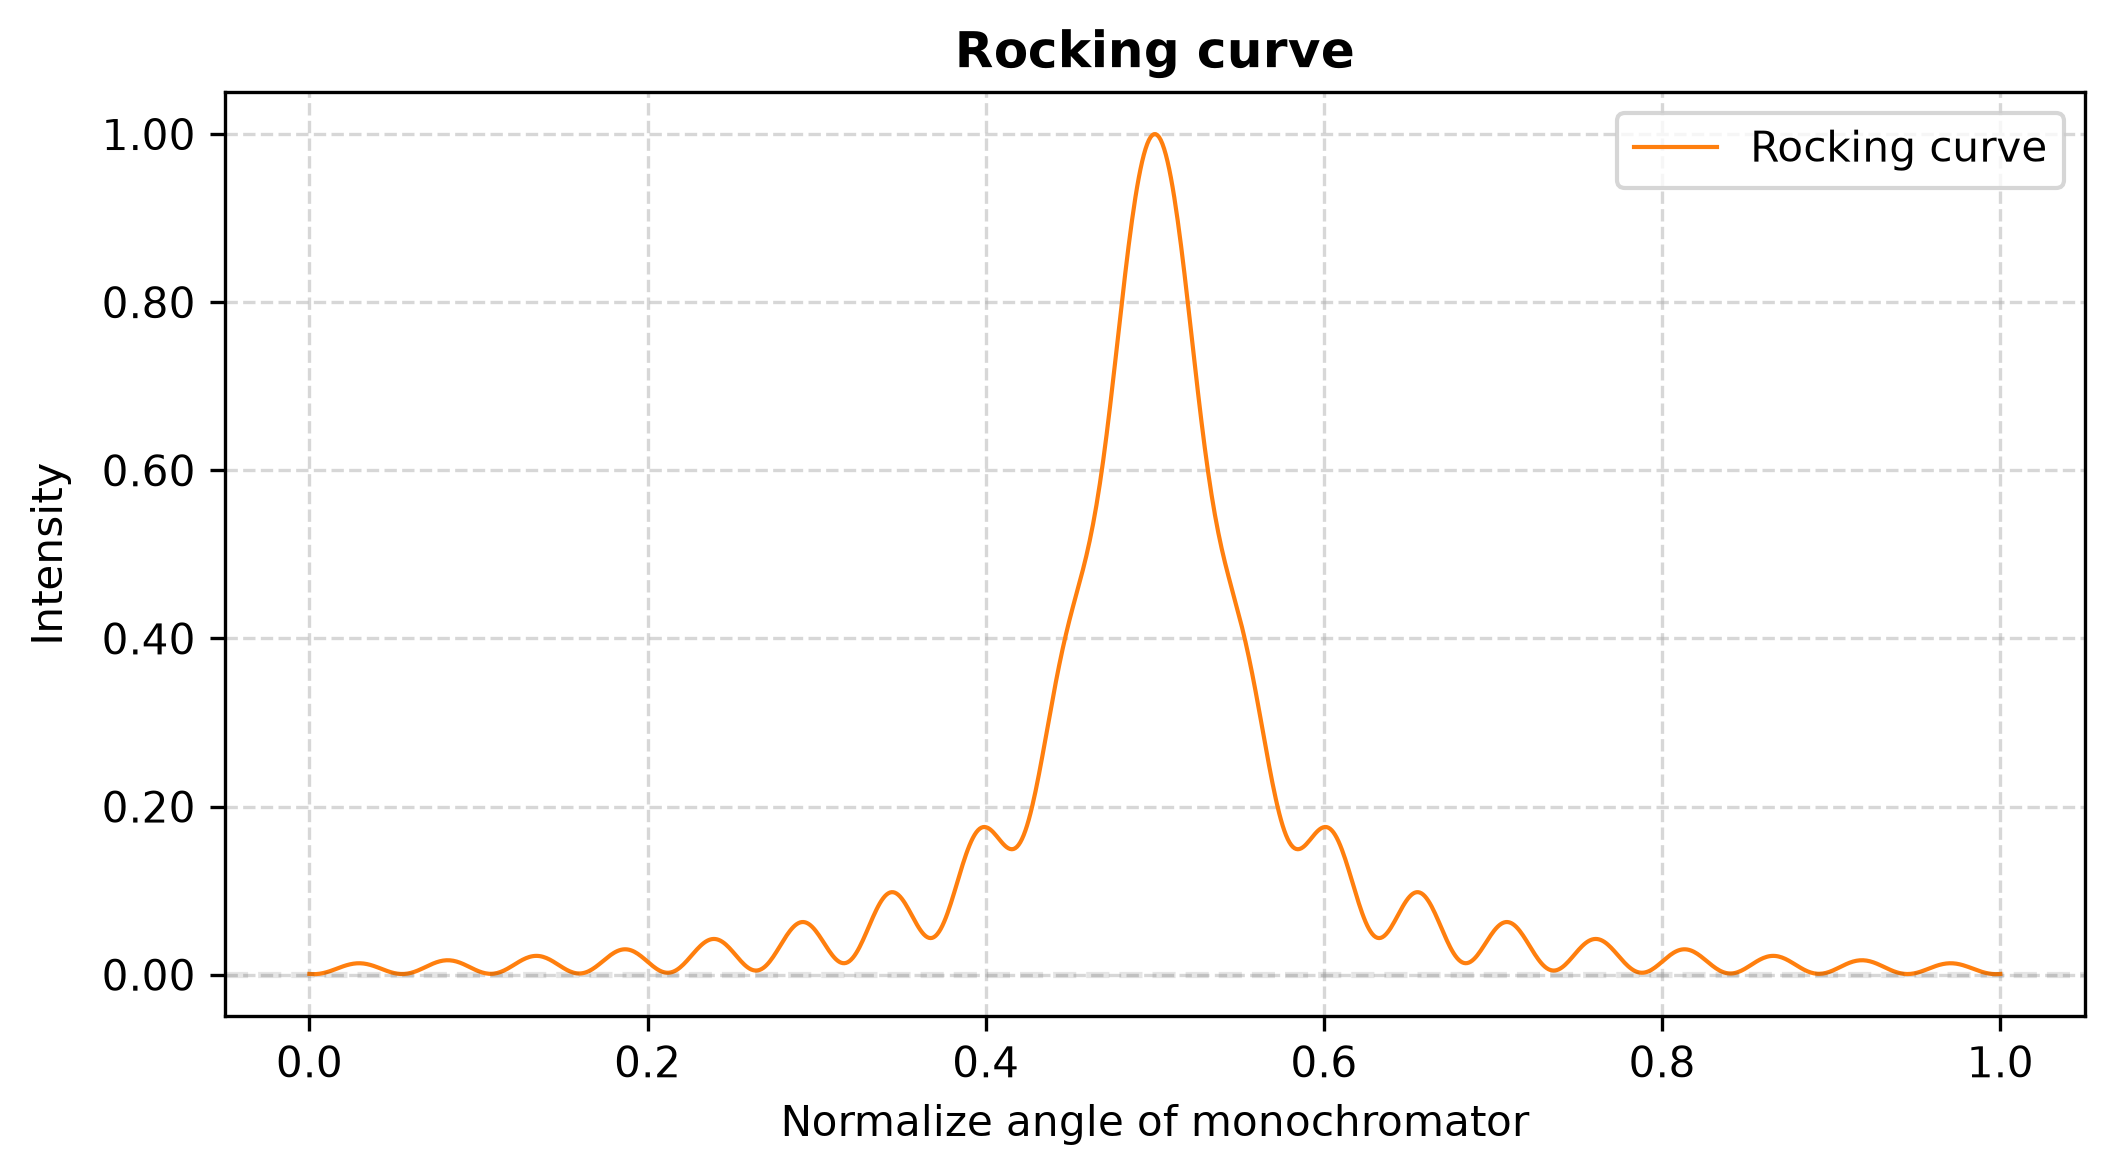
\includegraphics[width=0.85\textwidth]{img/cap 1/Rocking curve.png}
    \caption{Example of rocking curve with the angle of DCM normalize between 0 and 1, and the intensity peak normalize to 1}
    \label{fig:rocking curve}
\end{figure}

The largest peak in the graph corresponds to the angle that must exist between the two crystals to produce the maximum intensity.
The angle that produces the maximum beam intensity is not necessarily fixed, and if it were to move, it would cause the crystals to become misaligned.
Thermal variations, mechanical vibrations, and the hysteresis of piezoelectric actuators can alter the crystal alignment over time \cite{Proux2006,Stoupin2010}.

Peak intensity drift is a problem that cannot be solved by beam position control alone.
In fact, the position control system could maintain the correct location of the beam without ensuring the alignment of the monochromator, resulting in a degradation in intensity.
It is necessary to add a control system that takes care of tracking the intensity peak.

\section{Importance of Peak Intensity Tracking}

There are several reasons to operate at maximum beam intensity, some experiments actually require the highest available monochromatic photon flux. 
If the monochromator is not aligned correctly, some of the intensity will be lost before the beam reaching the sample.
Some experiments require counting photons until the required number is reached. 
If some photons are lost, the experiment will take longer to reach the required number of photons.

The stability of the system during experiments or beam scanning should not be underestimated.
Stability is also important during measurements that last several minutes or hours, or while the photon energy is scanned. 
If stability were to be lost, it would be difficult to compare experiments, which could change the interpretation of the data \cite{Proux2006,vanSilfhout2014,Quinn2021}.

The main goal of the thesis is to design a control system that not only finds the peak of intensity, but also follows it in case it moves.
This can be done by a feedback control loop which, based on the intensity produced, applies the right correction to change the angle between the two crystals of the monochromator in order to reach the peak intensity.

\section{Existing Beam Stabilization Solutions}

The problem of peak intensity oscillation has already been encountered and several solutions have emerged.
Some implemented solutions involve using position to change the intensity while others use components to directly change the intensity of the beam.
Changing the intensity directly via a monochromator is a non-trivial problem, since the intensity does not vary monotonically with the relative crystal angle.

Proux et al. \cite{Proux2006} describe their work done at the ESRF, specifically for a DCM cooled with liquid nitrogen.
The main idea of what they did is based on small adjustments using piezoelectric actuators and the use of lock-in to extract the gradient of the rocking curve.
The controller uses the gradient information to correct the angle between the monochromator crystals and keep it stable at the intensity peak.
The ESRF Monochromator Controller (MoCo) provides a related example of dedicated instrumentation \cite{MoCo2008}. 
MoCo provides three modes of operation: position, fixed intensity, and oscillation.
The latter injects a small disturbance to understand the gradient of the rocking curve through synchronous detection.

Stoupin et al. \cite{Stoupin2010} instead opted for another approach, namely the null-detection principle, for angular stabilization of optical components.
They were able to validate their proposal by testing with an angular stability of approximately $13\,\mathrm{nrad}$ RMS.
This demonstrates how sensitive the angle between the two crystals is and the usefulness of a control system even when the required corrections are very small.

Van Silfhout et al. \cite{vanSilfhout2014} proposed a system to simultaneously control both the intensity and the position of the beam.
To do this they used two independent systems, one for position and one for intensity.
This shows that the two problems, although dependent on each other, require distinct solutions, each with its own purpose.

Extremum-seeking, as mention before, can be used for beam stabilization too. 
In fact, Zohar et al. \cite{Zohar2016} used this approach to stabilize the beam intensity by introducing a small sinusoid to the piezoelectric
Although they did not directly modify the angle between the crystals of the monochromator, they managed to stabilize the intensity.
Their situation revolves around beam positioning through an aperture.
More recently, Quinn et al. \cite{Quinn2021} have implemented a combined control system at software level that allows both the position and the intensity of the beam to be managed simultaneously.

These work demonstrated the non-uniqueness of the solution for tracking the intensity peak.
The aim of this thesis is not to create a new solution, but based on what has already been done, implement it within the Beamline Enhanced Stabilization Technology (BEST) system \cite{BEST2024}.
With particular attention to the feedback control system and everything related to it.
The topics covered around the feedback control system will be: digital signal processing, controllers, delay introduced by the whole system (control, mechanism, actuator, etc...) and to the possible setting of parameters for different operating conditions.

\section{Feedback Control System}

The photon beam moves in time and for aiming it onto a target material, it requires a closed-loop feedback control system.
During the experiments the system must read the position of the beam from the beam and compute the correction needed for adjust the position of the photon beam.
The BEST system already has the position feedback control systems, but it cannot track the peak intensity of the photon beam.
The use of a feedback control approach has already been demonstrated, both for position control and for peak intensity tracking  \cite{Proux2006,MoCo2008,vanSilfhout2014,Quinn2021}.
Proportional-Integral-Derivative (PID) are controllers widely diffuse around different field and topics, from industrial to scientific domains. 
The key characteristics for his popularity are simplicity reliability and effectiveness.
A standard PID controller use the difference between the setpoint and the measured value for calculate the corrective control output and it is based on three distinct terms:

\begin{itemize}
    \item \textbf{Proportional (P):} Generates an output proportional to the current positioning error, scaled by a proportional gain factor.
    \item \textbf{Integral (I):} Accumulates past positioning errors over time to eliminate steady-state error and overcome system bias (with appropriate anti-windup mechanisms).
    \item \textbf{Derivative (D):} Evaluates the rate of change of the error signal to anticipate future trajectory shifts and damp transient responses.
\end{itemize}

The ideal continuous-time PID control function $u(t)$ can be expressed as:

\begin{equation}
    u(t) = K_p e(t) + K_i \int_{0}^{t} e(\tau) \, d\tau + K_d \frac{de(t)}{dt} 
\end{equation}

where $e(t)$ represents the positioning error, and $K_p$, $K_i$, and $K_d$ denote the proportional, integral, and derivative gains, respectively.

\section{Proposed Solution: Intensity Peak Tracking with the BEST system}


The thesis revolves around the integration of the peak intensity tracking system into the BEST system.
The system already created by ELS Instruments already has the position control system present but the peak tracking system discussed in this thesis is not present.
For reaching the goal of this thesis, it is needed to understand the Beamline Enhanced
Stabilization Technology (BEST) system first. 
It is then possible to achieve the goal, which is to add a peak intensity tracking system.

The BEST system architecture is composed by three main hardware modules: a \textit{TetrAMM}, a \textit{Central Unit} and a \textit{PreDAC}.

The primary control data flow operates as follows:
\begin{itemize}
    \item The \textit{TetrAMM} unit reads the photo-emitted currents from the beam position sensors, digitizes the signals, sends the 4 currents data to the \textit{Central Unit}.
    \item The \textit{Central Unit} converts the currents into positions and intensity, processes the feedback algorithm, calculate the necessary corrective displacements required to maintain target alignment and transmits control commands to the \textit{PreDAC}.
    \item The \textit{PreDAC} converts digital control commands from the The \textit{Central Unit} into high-precision analog voltage signals fed idrectly into the piezoelectric actuators.

\end{itemize}

\begin{figure}[htbp]
    \centering
    \begin{tikzpicture}[
        scale=0.85, transform shape,
        beam/.style={line width=1.5pt, orange!80!black},
        component/.style={draw, rectangle, rounded corners, thick, fill=blue!10, minimum width=2.2cm, minimum height=1.1cm, align=center, font=\small},
        bestblock/.style={draw, rectangle, dashed, thick, fill=red!5, minimum width=6.5cm, minimum height=2.0cm, align=center, font=\small},
        hardware/.style={draw, rectangle, thick, fill=gray!20, minimum width=2.4cm, minimum height=1.0cm, align=center, font=\small},
        cable/.style={thick, blue!50!black, -Stealth}
    ]

      % --- BEAMLINE LAYOUT ---
      \coordinate (source) at (0, {3.5 - 0.2*cos(10)});
      \coordinate (c1) at (3.2, 3.5);
      \coordinate (c2) at (5.8, 2.8);
      \coordinate (c3) at (5.8, 2.1);
      
      \coordinate (c1_bottom) at ($(c1) - ({0.2*sin(10)}, {0.2*cos(10)})$);
      \coordinate (c3_top) at ($(c3) + ({0.2*sin(28)}, {0.2*cos(28)})$);
      \coordinate (c2_bottom) at ($(c2) - ({0.2*sin(28)}, {0.2*cos(28)})$);

      \coordinate (det) at ($(c3_top) + ({2.2},{0})$);
      \coordinate (sample) at ($(det) + ({2.0},{0})$);

      % Draw X-ray beam path
      \draw[beam] (source) node[above, black, font=\bfseries] {Synchrotron Source} -- (c1_bottom);
      \draw[beam] (c1_bottom) -- node[above right, font=\footnotesize, black] {DCM} (c2_bottom);
      \draw[beam] (c2_bottom) -- (c3_top);
      \draw[beam] (c3_top) -- (det);
      \draw[beam] (det) -- (sample);

      % --- OPTICAL COMPONENTS (DCM & DETECTORS) ---
      \draw[thick, fill=cyan!30, rotate around={-10:(c1)}] ($(c1)+(-0.4,-0.2)$) rectangle ($(c1)+(0.4,0.2)$);
      \node[above=0.25cm, font=\small] at (c1) {Crystal 1 (Fixed)};

      \draw[thick, fill=cyan!30, rotate around={-28:(c2)}] ($(c2)+(-0.4,-0.2)$) rectangle ($(c2)+(0.4,0.2)$);

      \begin{scope}[shift={(c3)}, rotate=-28]
        \draw[thick, fill=cyan!30] (-0.4,-0.2) rectangle (0.4,0.2);
      \end{scope}

      % Ion Chamber / Detector (I0)
      \draw[draw, thick, fill=green!20] ($(det)+(-0.3,-0.6)$) rectangle ($(det)+(0.3,0.6)$);
      \node[above=0.6cm, font=\small, align=center] at (det) {BPM\\(Detector)};

      % Endstation / Sample
      \node[component] at (sample) {Sample /\\ Endstation};

      % --- ELS INSTRUMENTS BEST SYSTEM INTEGRATION ---
      \node[hardware] (predac) at (4.5, -0.6) {PreDAC\\(Actuator Module)};
      \node[hardware] (tetramm) at (8.2, -0.6) {TetrAMM\\(Readout Module)};

      \node[bestblock] (central) at (6.35, -4.0) {
        \textbf{ELS Instruments BEST Central Unit}
      };


      % --- CABLING & SIGNALS ---
      \draw[cable] (predac.north) -- node[right, font=\footnotesize] {Drive + Dither ($V$)} ($(c2)+(0,-0.8)$);
      \draw[cable] (det.south) -- node[right, font=\footnotesize] {Current Signals} (tetramm.north);
      \draw[cable, <->] (predac.south) -- node[left, font=\footnotesize] {Optical link} (predac.south |- central.north);
      \draw[cable, <->] (tetramm.south) -- node[right, font=\footnotesize] {Optical link} (tetramm.south |- central.north);

    \end{tikzpicture}
    \caption{Schematic layout of a synchrotron beamline optics and hardware integration using the BEST system. The X-ray beam reflects off the Double Crystal Monochromator (DCM), passes through the BPM for position and intensity readout, and reaches the endstation. Real-time position control loops executed on the Central Unit coordinate the PreDAC actuator module and TetrAMM readout module to keep position stable in a closed-loop fashion.}
    \label{fig:beamline_best_integration}
\end{figure}

The \textit{Central Unit} is composed by two main parts: a Field-Programmable Gate Array (FPGA), which is where run the real-time feedback control loop, and a industrial host PC.
The latter runs a custom graphical user interface (GUI) that allows you to view the beam position and modify the feedback control system.
The TetrAMM reads the currents produced by BPM and translates to digital signals and sends them to the Cental Unit.
The PreDAC on the other hand, reads the correction signal coming from the Central Unit and converts it into small analog voltage that move the actuators.
The three hardware modules are connected with a Small Form-Factor Pluggable (SFP) optical interfaces in order to have High-speed, low-latency and reduce noise pick-up inside the system.

The FPGA includes a soft-core processor that runs the control firmware, so the feedback loop can be executed at deterministic intervals while retaining the flexibility of a software-based control algorithm.

The method chosen for tracking the intensity peak is one of those mentioned above, which involves the insertion of a small dither signal, to the voltage that moves the piezoelectric actuator connected to the DCM.

Instead of calculating the intensity derivative from the raw noise data received from the TetrAMM, a pipeline consisting of digital filters and synchronous demodulation will be used.
First the intensity passes through a band-pass filter centered on the frequency of the dither signal.
Then the filtered signal is demodulated with a reference signal having the same frequency as the dither signal and finally it is filtered with a low-pass filter to obtain the intensity gradient, $\mathrm{d}I/\mathrm{d}\theta$.
Next, the gradient is sent to the PID, which will calculate the movement the actuator will have to make to reach the maximum intensity.

The time required to apply the dither signal and read its intensity response is considered delay time.
To this must be added the delay introduced by the filters.
This delay must be taken into account because demodulation is synchronous; otherwise, it would lead to incorrect demodulation, resulting in poor accuracy.
To overcome this problem, a routine for automatically calculating the phase delay has been included.
The routine includes in-phase, quadrature, and four-quadrant arctangent methods for calculating the phase delay.

Since the solution is composed of parameter-based methods, the ultimate goal is to make the parameters configurable.
The parameters in question are the amplitude and frequency of the dither signal, the filter coefficients, and the PID coefficients.
Starting from the parameterization made for the position control, it should be extended for the control on the intensity peak.
The design, implementation and validation will be explained in the next chapters.

\section{Thesis Outline}

The thesis is organized into five chapters. Chapter 2 reviews the feedback methods and signal-processing techniques used for beam stabilization and intensity tracking. Chapter 3 describes the proposed implementation within BEST, including the digital filtering pipeline, the PID control loop, and the automatic phase calibration procedure. Chapter 4 presents the validation of the system through simulation, together with the FPGA resource and timing checks and the analysis of the controller response. Finally, Chapter 5 discusses the conclusions of the work and the possible developments needed for testing the system on a physical beamline.

\newpage